%; whizzy chapter
% -initex iniptex -latex platex -format platex -bibtex jbibtex -fmt fmt
% 以上 whizzytex を使用する場合の設定。

%     Kansai Debian Meeting resources
%     Copyright (C) 2007 Takaya Yamashita
%     Thank you for Tokyo Debian Meeting resources

%     This program is free software; you can redistribute it and/or modify
%     it under the terms of the GNU General Public License as published by
%     the Free Software Foundation; either version 2 of the License, or
%     (at your option) any later version.

%     This program is distributed in the hope that it will be useful,
%     but WITHOUT ANY WARRANTY; without even the implied warranty of
%     MERCHANTABILITY or FITNESS FOR A PARTICULAR PURPOSE.  See the
%     GNU General Public License for more details.

%     You should have received a copy of the GNU General Public License
%     along with this program; if not, write to the Free Software
%     Foundation, Inc., 51 Franklin St, Fifth Floor, Boston, MA  02110-1301 USA

%  preview (shell-command (concat "evince " (replace-regexp-in-string "tex$" "pdf"(buffer-file-name)) "&"))
% 画像ファイルを処理するためにはebbを利用してboundingboxを作成。
%(shell-command "cd image200708; ebb *.png")

%%ここからヘッダ開始。

\documentclass[mingoth,a4paper]{jsarticle}
\usepackage{kansaimonthlyreport}
\usepackage{ascmac}

% 日付を定義する、毎月変わります。
\newcommand{\debmtgyear}{2008}
\newcommand{\debmtgdate}{18}
\newcommand{\debmtgmonth}{5}
\newcommand{\debmtgnumber}{13}

\begin{document}

\begin{titlepage}

% 毎月変更する部分, 本文の末尾も修正することをわすれずに

 第\debmtgnumber{}回 関西 Debian 勉強会資料

\vspace{2cm}

\begin{center}
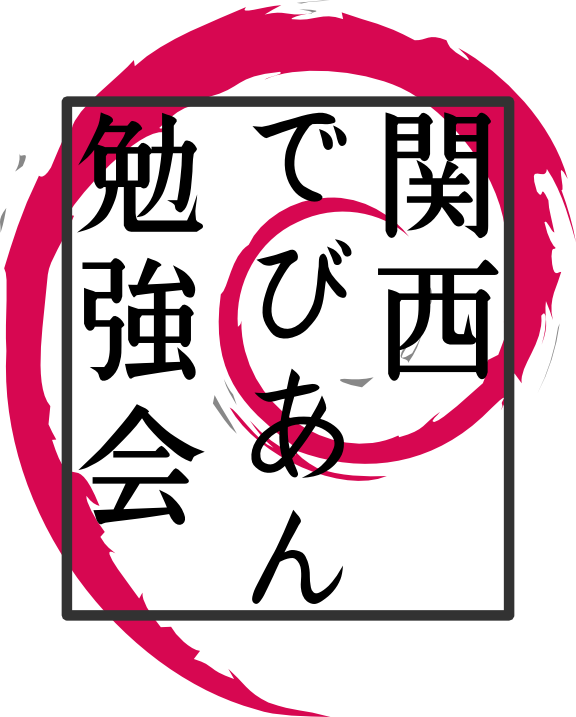
\includegraphics{image200802/kansaidebianlogo.png}
\end{center}

\begin{flushright}
\hfill{}関西 Debian 勉強会担当者 山下 尊也\\
\hfill{}\debmtgyear{}年\debmtgmonth{}月\debmtgdate{}日
\end{flushright}

\thispagestyle{empty}
\end{titlepage}

\dancersection{Introduction}{山下 尊也}
 
 関西 Debian 勉強会はDebian GNU/Linux のさまざ
 まなトピック(新しいパッケージ、Debian 特有の機能の仕組、Debian 界隈で起
 こった出来事、などなど)について話し合う会です。

 目的として次の三つを考えています。
 \begin{itemize}
  \item MLや掲示板ではなく、直接顔を合わせる事での情報交換の促進
  \item 定期的に集まれる場所
  \item 資料の作成
 \end{itemize}

 それでは、楽しい一時をお楽しみ下さい。

\newpage

\begin{minipage}[b]{0.2\hsize}
 {\rotatebox{90}{\fontsize{80}{80}
{\gt 関西デビアン勉強会}}}
\end{minipage}
\begin{minipage}[b]{0.8\hsize}
\hrule
\vspace{2mm}
\hrule
\setcounter{tocdepth}{1}
\tableofcontents
\vspace{2mm}
\hrule
\end{minipage}

\dancersection{最近のDebian関係のイベント報告}{山下 尊也}
\subsection{第12回 関西 Debian 勉強会}
2008年4月29日に「第12回 関西 Debian 勉強会」を行いました。
勉強会は、合計21名の参加でした。

インターネット回線や部屋などを手配して頂き、
姫路獨協大学の園田先生ありがとうございました。

有志により勉強会とは別に、観光ツアーも行われ、
みなさん、姫路城の方を観光なされたみたいです。

今回、インターネット環境が充実していたため、
初めて ustream.tv による中継を行ったり、
東京から DebianJP 会長である上川さんが来て頂いたりと、
非常におもしろい勉強会になったと思っています。

\subsubsection{発表内容}

\begin{itemize}
 \item Windows な PC でも Debian を楽しもう 名村さん
 \item Debian GNU/kFreeBSD 大浦さん
 \item はじめてのsid たかや
\end{itemize}

Windows な PC でも Debian を使う手段として、名村さんに
coLinux について説明して頂きました。
質問では、Cygwinよりも速度的に速いの?
や、どのような仕組みになっているのか?
などの内容についての質問がありました。
また、名村さんによる coLinux 実践編を予定していますので、
今後も楽しめそうです。

2人目のDebian GNU/kFreeBSDについて大浦さんにご紹介して頂きました。
インストールから始まり、実際に X が動いてる画面を見ると、
会場から声があがり、ustream.tv先のやまねさんが、
2chを見るためのソフトである、jdが動くのか?
と言うことで、実際に jd をインストールし、動く姿が確認されました。
大浦さん、やまもとさん、岩松さんによる Debian GNU/kFreeBSD についての
文章作成も進んでるようなので、今後も Debian GNU/kFreeBSD から目が離せま
せん。

カーネル周りの話が2つあり、会場、そしてインターネットからもたくさ
んの質問があっため、私のセクションは、かなり短くなってしまいました。
カーネル周りの話などは、多くの質問が予想出きるので、
今後は、セッション時間の調整や、セッション数の調整が必要になってくると
考えています。
また、時間の余裕がなく、資料不足な点もあったので、
今後、資料を追加していく予定です。

%%% nogata jun
\dancersection{ustream.tvを使った関西Debian勉強会中継の裏側}{野方 純}

\subsection{はじめに}

4月29日の第12回関西Debian勉強会は、姫路での開催ということもあり、
ustream.tvのサービスを利用したインターネットビデオ中継を行いました。

ustream.tvはWindowsやMacの環境からは比較的簡単に利用できるようになってい
ますが、Debianでは少しつまづくところがあったので、その辺りを中心にTipsな
どを交えながら述べたいと思います。

\subsection{ustream.tvについて}

\subsubsection{ustream.tvとは}

ustream.tv(\url{http://www.ustream.tv/})とはWebブラウザとAdobe Flash
Playerを使いインターネットビデオ中継を行うことができるwebサービスです。
特徴としては、以下のようなものがあります。

\begin{itemize}
 \item WebブラウザとFlashプラグインとカメラがあればどこでもストリーミン
       グ中継ができる。
 \item ストリーミング中継は同時に録画でき、すぐにWeb上で公開できる。
 \item チャットがあるので視聴者も参加でき講演者は反応をダイレクトに知ることができる。
\end{itemize}

手軽にストリーミング中継ができることから、オープンソース系の勉強会では最
近よく使われるサービスです。

\subsubsection{ustream.tvを使って中継をするまでの流れ}

中継をするまでの流れを \url{http://www.ustream.tv/get-started} から引用
すると、このような感じになります。

\begin{enumerate}
 \item ustreamアカウントを作る(アカウントのある人はログインする)
 \item カメラをPCに接続する。
 \item ログインして"My Show"をクリック。
 \item "Name Your Show"にストリーミングの番組名を入力して"BROADCAST NOW"
       ボタンをクリック。
 \item Flashプラグインに「www.ustream.tvのカメラおよびマイクへのアクセス
       を許可しますか?」と尋ねられたら「許可」をする。
 \item "START BROADCAST"ボタンをクリックして放送開始。
\end{enumerate}

\subsubsection{中継をするために用意するもの}

ustream.tvの中継に必要なものをまとめました。必須なものについては、Debian
をデスクトップ環境にて利用されている方は普段使っているものばかりだと思い
ます。

\begin{itemize}
 \item 必須
       \begin{itemize}
	\item インターネット接続環境
	\item Debianがインストールされたマシン\verb|;)|
	\item Adobe Flashプラグイン
	\item Webブラウザ
	\item カメラ
	\item マイク
       \end{itemize}
 \item あれば便利
       \begin{itemize}
	\item オーディオミキサー
	\item IRCクライアント
       \end{itemize}
\end{itemize}

\subsection{実際に中継をする}

以上で中継に必要なものと手順がわかったので実際に中継してみました。

\subsubsection{中継ができた人とできない人がいた}

中継の実験をT氏と行っていましたが、筆者はほとんどトラブルもなく中継を行
うことができたのに対し、T氏は中継をすることができませんでした。
その理由を探っていくとどうやらFlash Playerに原因があることがわかりました。

\subsubsection{Flash Playerについて調べる}

\begin{description}
 \item[Debian GNU/Linux(i386)で使えるFlash Playerについて]

Debianで使えるFlash Playerは3つ存在しますが、ustream.tvのサービスを利用
するにはSWF V9が必要なので、フリーソフトウェアのGnashとSwfdecを使うこと
ができませんでした。ですのでAdobe Flash Playerを使用することになります。

Adobe Flash Player(SWF V9) | プロプライエタリソフト | non-freeセクション
を追加してflashplugin-nonfreeをインストールするほかに、iceweasel2を使っ
ていればユーザーディレクトリに自動インストールも可。

Gnash(SWF V7) | フリーソフトウェア(GPL V3) | aptitude install mozilla-plugin-gnashでインストール可
Swfdec(SWF V7) | フリーソフトウェア(GPL V2) | aptitude install swfdec-mozillaでインストール可

 \item[Adobe Flash Playerの制限]

Adobe Flash Playerは他のOSとほぼ同じバージョンなので、
同じように扱えるように見えますがLinux版には制限があります。

\begin{enumerate}
 \item 対応しているビデオAPIがVideo4Linux(V4L)のみ。(Kernel 2.6以降では
       V4L2が標準。V4Lは互換レイヤーで対応)
 \item サウンドの入出力にALSAを利用しているがサウンドデバイスを直接扱う。
 \item インプットメソッド(IM)の扱いがGTKのIM周りを考慮していない。
\end{enumerate}


3はさておき、1と2の理由により使用するデバイスで
中継ができた人とできない人に分かれました。

\end{description}

\subsection{Adobe Flashで利用できるデバイスを考える}

使用できるデバイスに制限があるということが分かったので、Adobe Flashで使
えるデバイスについて考えてみます。

\subsubsection{カメラ}

PCに直接接続できるカメラは大きくわけて、このようなものがあります。

\begin{itemize}
 \item Webカメラ
       \begin{itemize}
	\item USB Video Class対応カメラ(linux-uvc)
	\item USB Video Class非対応カメラ(gspca, ov511, qc-usb)
       \end{itemize}
 \item DV(デジタルビデオ)カメラ
       \begin{itemize}
	\item IEEE1394接続
	\item USB接続
       \end{itemize}
\end{itemize}

USB接続のカメラでWebカメラと呼ばれるものは、USB Video Class対応のものと
非対応なものでわけることができます。まずUSB Video Class対応カメラはドラ
イバのlinux-uvcがV4L2しか対応しておらずV4L互換レイヤーをサポートしていな
いのでV4Lしか使えないFlashでは使うことができません。
\footnote{The Flashcam Project
(\url{http://www.swift-tools.net/Flashcam/}) のflashcamを利用すればFlash
でもlinux-uvcカメラが使えるようです(未確認)}


USB Video Class対応カメラかそうでないかの見分け方は、

\begin{enumerate}
 \item 解像度が130万画素以上。
 \item Windowsドライバ不要とうたっている。
\end{enumerate}

どちらかに当てはまれば、UVC対応と見ればほぼ間違いないでしょう。

USB Video Class非対応のカメラについてはMicrosoft VX-1000とLogitech
Quickcam Expressの2種類使用しましたが、ドライバがV4Lに対応していたので楽
に使うことができました。ただUVC非対応のカメラはどのドライバに対応してい
るのか自分で見分けなければいけないことと、画素数が30万〜50万クラスのもの
しかないので画質に不満が出るかもしれません。


デジタルビデオ(DV)カメラについてですが、IEEE1394接続のカメラは転送される
データ形式がDV形式でV4Lは直接扱えないのでDV4Linuxを経由して使う必要があ
ります。映像についてはカメラとしての機能がしっかりしているので不満はない
と思います。


USB接続のDVカメラについては他のOSでは使用したとの記事を見かけたのですが、
まだ使用したことがないのでdebian上で使えるかどうかわかりません。


Linuxで使えるカメラについてまとめましたが、現時点では一長一短がありコレ
といっておすすめできるものがありません。なので、まだまだ試行錯誤は続くと
思われます。

\subsubsection{カメラの設定について}

使用したカメラの設定について述べます。

\begin{description}
 \item[Microsoft VX-1000/Logitech Quickcam Expressの設定] 

それぞれUVC非対応のカメラなので、VX-1000はgspca、
Quickcam Expressはqc-usbのカーネルモジュールを使います。
標準のカーネルを使っている人は自分の使っているカーネル用の
カーネルモジュールが用意されるので、それをインストールしてください。

自分で作ったカーネルを使っている人はmodule-assitantを使って
カーネルモジュールパッケージをインストールします。

\begin{commandline}
# aptitude install module-assistant
# m-a a-i gspca (VX-1000の場合)
# m-a a-i qc-usb (Quickcam Expressの場合)
\end{commandline}

あとはカメラを接続してブラウザでustream.tvに
アクセスするだけで使うことができました。

 \item[IEEE1394接続のDVカメラの設定]

IEEE1394接続のDVカメラは、DV4Linuxを経由して
ブラウザを起動する必要があります。

 \item[DV4Linuxのインストール]

DV4Linuxはdebianパッケージになっていないので
配布元(\url{http://dv4l.berlios.de/})からソースを
ダウンロードしてインストールする必要があります。

パッケージ作成練習と自分で使うために作った
sid用debianパッケージを作りましたが、きちんと
作っていないのでリスクを覚悟できる人だけ使ってください。

\url{http://regret.nofuture.tv/packages/dv4l_1.0-1_i386.deb}

\begin{commandline}
$ tar xvfz dv4l-1.0.tar.gz
$ cd dv4l-1.0/
$ ./configure
$ make
$ sudo make install
\end{commandline}

DV4Linuxをインストールするとvloopback
\footnote{仮想ビデオデバイスを作るカーネルモジュール。 
DV4Linuxとは別途インストールする必要があります。
Vloopback - Oss4art (\url{http://megaui.net/oss4art/wiki/Vloopback})}
を経由してDVカメラとデータをやりとりをするdv4lと、
直接DVカメラとやりとりするdv4lstartの2種類が
インストールされますが、dv4lは使うと画像が途切れ途切れに
送られてきて不安定なのでdv4lstartを使用します。

dv4lstartを使ってブラウザを起動するには、このようにします。

\begin{commandline}
$ dv4lstart iceweasel
\end{commandline}

統合デスクトップ環境を使っている方は
ショートカットアイコンを作っておくと便利です。

\end{description}

\subsubsection{参考}

\begin{itemize}
 \item DV4Linux (\url{http://dv4l.berlios.de/})
 \item ビデオキャプチャ:デバイス編 - Oss4art
 (\url{http://megaui.net/oss4art/wiki/%E3%83%93%E3%83%87%E3%82%AA%E3%82%AD%E3%83%A3%E3%83%97%E3%83%81%E3%83%A3:%E3%83%87%E3%83%90%E3%82%A4%E3%82%B9%E7%B7%A8>})
 \item Debian の最新 Linux kernel で DV 関係が全滅の件 - ほげめも
       (\url{http://www.keshi.org/blog/2007/08/debian_linux_kernel_disaster.html})
\end{itemize}

\subsection{サウンド}
基本的にはALSAで録音再生できるものであれば種類を問いませんが、AdobeFlash
はALSAの標準的なPCMデバイス名の =default= を使わず、最初に認識されたサウ
ンドのハードウェアにつけられるデバイス名 =hw:0,0= を利用して録音再生しよ
うとします。ですのでUSBサウンドなどを接続して複数のサウンドカードを使用
している場合には注意が必要です。

筆者の場合、USBサウンドユニットをALSAの設定ファイルの.asoundrcで
=default= に定義して使っていましたが、これではまったくFlashは録音再生を
してくれないので、サウンドカード認識の順番を変更することで対処しました。

\subsubsection{サウンドカードの認識順を変更する}

サウンドカードの認識順を変更方法は、/etc/modprobe.d/soundを変更する事に
よって行います。

サウンドカードの設定はこのような感じで指定するので

\begin{commandline}
alias snd-card-(番号) snd-(ドライバ名)
options snd-card-(番号) index=(番号)
\end{commandline}

実際にはこうなります。

\begin{commandline}
# alias snd-card-0 snd-hda-intel           元々の設定をコメントアウト
# options snd-hda-intel index=0 model=will 元々の設定をコメントアウト
alias snd-card-0 snd-usb-audio
options snd-usb-audio index=0
\end{commandline}

詳しい設定方法についてはカーネルソース付属のドキュメント、
Documentation/sound/alsa/ALSA-Configuration.txtを参照してください。

Flashのサウンド入出力について、contribセクションにある
flashplugin-nonfree-extrasoundパッケージを使えば、サウンドサーバーの
PulseAudioやEsound経由で変更できるようですが、筆者はデスクトップ環境に
KDEを使用しているので未確認です。

\begin{itemize}
 \item Flash Player:Additional Interface Support for Linux - Adobe Labs
(\url{http://labs.adobe.com/wiki/index.php/Flash_Player:Additional_Interface_Support_for_Linux})
 \item PulseAudio - Revolution Linux OpenSource projects
(\url{http://pulseaudio.revolutionlinux.com/PulseAudio})
\end{itemize}

\subsection{本番で中継をするにあたってのTips}

ustream.tvで中継をするにあたり、障害になるデバイスの問題も解決できたので
基本的にはこれで中継を行うことができます。しかし、よりよい中継を行うため
に少しこだわってみます。

\subsubsection{マイクにこだわる}

ustream.tvでの中継を見ていると、マイクの音が小さすぎて会場で何を言ってい
るのかさっぱりわからない事があります。そうすると見ている方としては興ざめ
してしまうので、会場の音をきちんと拾うためにマイクにこだわってみましょう。

姫路からの中継では手持ちのサウンドミキサーとマイクを使用しましたが、サウ
ンドミキサーは6〜8000円前後、マイクは一本3000円程度のものでも十分なので
用意しておくとよいでしょう。

BEHRINGERというメーカーのULTRAVOICE XM1800Sというマイクは3本セットで4000
円前後と非常にお買い得なのですが、マイクが複数本あると講演者と会場の音と
いうように分けて音を拾うことができるのでおすすめです。

\subsubsection{IRCクライアントでチャットに接続する}

ustream.tvはビデオストリーミングだけでなくIRCによるチャットも用意されて
います。しかし用意されているチャットクライアントはFlashで作られており日
本語がうまく扱えません。

ということでストレスをためながらチャットをするよりも、使い慣れたIRCクラ
イアントを使ってチャットをするほうがストレスもたまらず、ログなども取れた
り便利なので、ustream.tvのIRCサーバーに接続する設定を書いておきます。

\begin{commandline}
サーバー名 | chat1.ustream.tv
ポート | 6667
文字コード | UTF-8
ユーザー名 | アカウントがある人はustreamアカウント名。なければ空にしておきます。
ニックネーム | 適当なニックネーム。アカウントのない人は、チャンネルに存
在しないもの以外にustreamアカウントにも存在しない
ものでないと使えません。
サーバーパスワード | ustreamアカウントのパスワード。アカウントのない人は必要ありません。
チャンネル名 | 中継アドレスのchannel以下に#をつけたもの。たとえば関西Debianの中継チャンネルに入るには
http://www.ustream.tv/channel/kansaidebian のkansaidebianの頭に#をつけて#kansaidebianというふうに指定します。
\end{commandline}

\begin{description}
\item[会場でチャットに参加している人も中継役]
ustreamのチャットは中継を見ながらチャットしているので当然ながら
講演に対しての質問などの意見が出てきます。
ですが講演者が必ずしもチャットを見ているわけではないので、
会場でチャットに参加している人がいるなら、適当なころ合いを見計らって
チャットで出た質問などを視聴者に代わってしてあげてください。
\end{description}

そうすると会場はもちろん、インターネットを通じて見ている人も
かなり盛り上がることは間違いないです。

\subsubsection{画面を中継するには?}

今までカメラを使っての中継を書いてきましたが実は/dev/videoに
出力できるものなら、なんでも中継することができます。
ということでPCの画面を中継することもScreencast4Linuxを使えばできます。

ちなみにScreencast4Linuxはまだdebianパッケージにはなっていません。
カーネルモジュールをパッケージにする方法がわからないので誰か挑戦してみて!

\begin{itemize}
 \item Screencast4Linux: LinuxのX Window上で手軽に
       スクリーンキャスト(\url{http://yanbe.org/screencast4linux/})
\end{itemize}

\subsection{最後に}

本来ならばここまで大きくなることもなかったのですが、
Adobe Flash Playerの奇妙な仕様によりこんなに長くなってしまいました。

Adobeも「Open Screen Project」の一環として仕様やAPIの利用制限を
撤廃したので、自由なソフトウェアのFlash Playerが発展し、
早くこのようなバッドノウハウに頼らなくなればと思っています。

\subsection{資料}

\subsubsection{ビデオデバイス周り}

Main Page - V4LWiki(\url{http://linuxtv.org/v4lwiki/index.php/Main_Page})\\
Video4LinuxのWiki。Linuxのビデオデバイス周りの情報は一通り揃っています。

Welcome to QuickCam Team! - QuickCam Team(\url{http://www.quickcamteam.net/})\\
Logitech Quickcam Teamのまとめサイト。ドライバの情報がまとまっています。

VideoFourLinuxLoopbackDevice \verb|<| Motion \verb|<| TWiki(\url{http://www.lavrsen.dk/twiki/bin/view/Motion/VideoFourLinuxLoopbackDevice})\\
仮想ビデオデバイスvloopbackのサイト

AVLD - Another Video Loopback Device(\url{http://allonlinux.free.fr/Projets/AVLD/})\\
もう一つの仮想ビデオデバイスの実装。

gstfakevideo(\url{http://code.google.com/p/gstfakevideo/})\\
gstreamerに流すための仮想ビデオデバイス。gstreamerは鼻血が出るほどむずか
しい。

Screencast4Linux: LinuxのX Window上で手軽にスクリーンキャスト
(\url{http://yanbe.org/screencast4linux/})\\
PCの画面をスクリーンキャストする。

DV4Linux(\url{http://dv4l.berlios.de/})\\
DVカメラとV4Lとやりとりするラッパーソフト。

The Flashcam Project(\url{http://www.swift-tools.net/Flashcam/})\\
UVCカメラとV4Lをやりとりするラッパーソフト。

\subsubsection{その他}

FrontPage - UstreamまとめWiki(\url{http://usy.jp/ustream/index.php?FrontPage})\\
ustream.tvで中継をするためのノウハウを集めたWiki。

ustream.tvからsmilevideoにアップロードするための講座(\url{http://www.ustream.tv/recorded/379002})\\
ドワンゴの溝口氏によるustream.tvで録画したflvをffmpegを使ってエンコード
してニコニコ動画のsmilevideoにアップロードするまでの講座。

表現のためのオープンソースソフトウェア - Oss4art(\url{http://megaui.net/oss4art/wiki/})\\
EffecTV開発者のふくち氏によるLinuxマルチメディア系の情報を集めたWiki。

HowtoCast - dcastkit - Trac(\url{https://ssl.keshi.org/projects/dcastkit/trac.fcgi/wiki/HowtoCast})\\
八重樫氏製作によるDebian Liveベースのライブストリーミングに特化した
LiveCD dcastkitを使ったストリーミング方法。

Penguin.SWF(\url{http://blogs.adobe.com/penguin.swf/})
AdobeのLinux用Flash開発者のblog

Adobe Bug and Issue Management System(\url{https://bugs.adobe.com/flashplayer/})
Flash Playerのバグトラック。まだできて間もないのであまりバグが登録されていません。

\dancersection{Debian で始める Emacs エディタ}{木下 達也}
\subsection{GNU Emacsとは}
GNU Emacsは、拡張・カスタマイズが可能なテキストエディタです。

GNUシステムの構成要素として1984年から開発が始まり、
現在もなお愛され続けています。

テキストエディタとしての基本的な機能に加えて、
複数の「バッファ」それぞれに応じた「モード」、
キー割り当てのカスタマイズ、Emacs Lispによるプログラミングが可能、
といった特徴があります。

その柔軟性は、文書作成、コーディングという用途に留まらず、
メール送受信、ウェブブラウズなどもこなせるほどです。

\subsection{Emacsのインストール}
\subsubsection{Debianパッケージ}

Debianではemacsパッケージをインストールすれば、Debian標準の
Emacsパッケージ(etchではemacs21、lennyではemacs22)がインストールされます。

\begin{commandline}
# apt-get install emacs
\end{commandline}

ウィンドウアプリケーションとして動かすのではなく、
端末でのみ利用したいのであれば、代わりに-noxパッケージ
(etchではemacs21-nox、lennyではemacs22-nox)を選べば、
依存関係が少なく、インストールサイズが小さくて済みます。

\subsubsection{Unicode日本語対応}

emacs21では、Unicode (UTF-8)日本語対応のためには、
別途mule-ucsパッケージが必要です。
(emacs22ではmule-ucs無しでも対応)

\begin{commandline}
# apt-get install mule-ucs
\end{commandline}

mule-ucsを有効にするには、設定ファイルのサンプル
\verb|/usr/share/doc/mule-ucs/examples/dot.emacs.ja|の内容を、
\verb|~/.emacs|の先頭の方に貼り付けておくとよいでしょう。
(emacs22でも有用な設定が含まれています)

注: mule-ucsを有効にする際には、やや時間がかかります。
また、\verb|~/.emacs|自身はUTF-8にしないように。
\verb|~/.emacs|読み込み前に環境変数でmule-ucsを有効にする方法もあります。
\verb|/usr/share/doc/mule-ucs/README.Debian|を参照。

\subsection{Emacsの利用法}

起動方法:

\begin{commandline}
emacs                 	通常起動
emacs -nw             	端末内で起動
emacs -q              	~/.emacsを読まずに起動
emacs -q -no-site-file	startupファイルを読まずに起動 (emacs22なら-Qでも可)
\end{commandline}

キーボード操作に慣れることで、Emacsをより快適に使えるようになります。

\begin{commandline}
C-x     Ctrlキーを押しながらx
M-x     ESCを押してからx  (またはAltキーを押しながらx)

ESC     EscキーまたはC-[
TAB     TabキーまたはC-i (字下げや補完に使う)
RET     EnterキーまたはC-m (改行と同時に字下げする場合にはC-j)
DEL     Back spaceキー
SPC     スペースキー

C-x C-c         Emacsを終了

C-p  上へ       C-n  下へ
C-b  左へ       C-f  右へ
C-a  行頭へ     C-e  行末へ

DEL     手前1文字を削除 (C-hはデフォルトではhelp-command)
C-d     1文字を削除
C-k     行末まで削除
C-o     行末までを次の行へ (改行を挿入、位置はそのまま)

C-x C-f         ファイルを読み込む
C-x C-s         ファイルを保存
C-x i           現在位置にファイルの内容を挿入
C-x C-w         別ファイルへ保存

C-x RET f       現在のバッファのcoding system(文字コード)を設定
C-x RET c       次に実行するコマンドのcoding systemを設定

C-v 次ページへ  M-v 前ページへ
M-< 先頭へ      M-> 末尾へ

C-s  前方検索   C-r  後方検索  (M-付きで正規表現)
M-%  置換  (C-付きで正規表現)

C-SPC マーク
C-w カット   M-w コピー   C-y ペースト

C-g     処理を中断
C-x u   Undo
C-l     現在行を中央にして再表示

C-x b バッファ移動   C-x k バッファ削除

C-x (   キーボードマクロ記録開始
C-x )   キーボードマクロ記録終了
C-x e   キーボードマクロ実行

C-x 2   ウィンドウ分割
C-x 1   他のウィンドウを削除
C-x 0   現在のウィンドウを削除

M-x     コマンド実行(Lisp関数を呼び出し)
M-:     ミニバッファで入力してLisp式を評価
C-x C-e 手前のLisp式を評価 (*scratch*ではC-jで評価・表示)
M-!     外部コマンド実行 (C-u付きで出力を現在位置へ挿入)

M-x help RET    ヘルプ
M-x info RET    マニュアル
M-x apropos RET 関数、変数等の名前を検索

\end{commandline}

カスタマイズ例:

\begin{commandline}
(global-set-key "\C-h" 'delete-backward-char)
(global-set-key "\C-ch" 'help-command)
(global-set-key "\C-z" 'scroll-down) ;; C-x C-z to use suspend/iconify
(global-set-key "\C-cg" 'goto-line)
(if (locate-library "iswitchb") (require 'iswitchb))
(if (fboundp 'iswitchb-default-keybindings) (iswitchb-default-keybindings))
(global-set-key "\C-cb" 'switch-to-buffer)
(setq visible-bell t)
(setq inhibit-startup-message t)
(if (fboundp 'menu-bar-mode) (menu-bar-mode -1))
(if (fboundp 'tool-bar-mode) (tool-bar-mode -1))
(if (fboundp 'auto-compression-mode) (auto-compression-mode 1))
\end{commandline}

\subsection{add-onパッケージ}

Emacs標準の機能だけでなく、さらに追加できるEmacs Lispパッケージがたくさんあります。

2008-05-13時点のDebian sidで、usr/share/emacsを含むパッケージ:

\begin{commandline}
# apt-file update
$ apt-file search usr/share/emacs | awk '{print $1}' | sort -u | cat -n
     1  a2ps:
     2  acl2-emacs:
     3  ada-mode:
     4  afnix:
     5  anthy-el:
     6  apel:
[...]
   256  yatex:
   257  yc-el:
   258  yorick-data:
   259  zenirc:
\end{commandline}

個人的なお勧め・注目パッケージ:

\begin{itemize}
 \item メールクライアント: mew, mew-beta, wl, wl-beta
 \item 引用ツール: mu-cite
 \item スケジュール管理: mhc, planner-el
 \item ウェブブラウザ: w3m-el, w3m-el-snapshot
 \item 日本語入力: ddskk, prime-el
 \item 辞書検索: lookup-el
 \item ローマ字での日本語検索: migemo
 \item 編集支援: muse-el, auctex, yatex
\end{itemize}

\subsection{emacsenパッケージ}

Debian sidに現時点で存在するemacsenパッケージ:

\begin{itemize}
 \item emacs22 (emacs22, emacs22-gtk, emacs22-nox)
 \item emacs21 (emacs21, emacs21-nox)
 \item xemacs21 (xemacs21-mule, xemacs21-mule-canna-wnn, xemacs21-gnome-mule,\\
       xemacs21-gnome-mule-canna-wnn, xemacs21-nomule, xemacs21-gnome-nomule)
\end{itemize}

非公式パッケージとして、Romain Francoiseさんによる
emacs-snapshotパッケージ(CVS版 Emacs 23.0.x)もあります。(\url{http://emacs.orebokech.com/})

Emacs Lisp add-onパッケージでは、emacsenそれぞれに応じた処理
(バイトコンパイル等)はインストール時に実施されるので、
パッケージはほぼ共通のものが使えます。

\dancersection{今後の予定}{山下 尊也}

\subsection{次回}
次回は、2008年6月29日に福島区民センター
\footnote{\url{http://www.city.osaka.jp/shimin/shisetu/01/fukushima.html}}
にて行なう予定です。

\subsection{OSC 2008 Kansaiについて}
今年のOSC Kansaiの日程が決まりました。
7月18,19日(金・土)に行なわれます。

関西 Debian 勉強会として決まっているのは、
以下の通りです。

\begin{itemize}
 \item 18日に参加出来る方が多ければ、18日,19日両日参加する
 \item セッション時間は、2時間頂き、通常とほぼ同様の勉強会を開催する
 \item ブース担当と、セッション担当に分ける
\end{itemize}

\subsection{KDRのおしらせ}
関西Debian勉強会の有志で
関西Debian勉強会とは独立した形で、
週に一度、読書会(KDR)を開いています。
詳しくはKDR公開用ページ\footnote{\url{http://qwik.jp/kdrweb/}}をご覧下さ
い。

% \dancersection{メモ}{}
% \mbox{}\newpage
 
\printindex
 \cleartooddpage

 \begin{minipage}[b]{0.2\hsize}
  \rotatebox{90}{\fontsize{80}{80} {\gt 関西デビアン勉強会} }
 \end{minipage}
 \begin{minipage}[b]{0.8\hsize}

 \vspace*{15cm}
 \rule{\hsize}{1mm}
 \vspace{2mm}
 
\includegraphics[width=2cm]{image200502/openlogo-nd.eps}
 \noindent \Large \bf Debian 勉強会資料\\ \\
 \noindent \normalfont \debmtgyear{}年\debmtgmonth{}月\debmtgdate{}日 \hspace{5mm}  初版第1刷発行\\
 \noindent \normalfont 関西 Debian 勉強会 (編集・印刷・発行)\\
 \rule{\hsize}{1mm}
 \end{minipage}

\end{document}
